\fancyhead[LE,RO]{Ionszelektív elektródok -- ,,SZEL''}
\fancyhead[LO,RE]{\thesection}
\fancyfoot[LE,RO]{\thepage}
\fancyfoot[RE,LO]{\emph{Fizikai Kémia gyakorlatok gyógyszerész hallgatóknak}}

\setcounter{section}{5}
\section{Szelektivitási együttható meghatározása}
\subsection{Bevezetés}

Az ionszelektív elektródok olyan potenciometriás érzékelők, melyek valamely ion aktivitásának többé-kevésbé szelektív meghatározását teszik lehetővé.
Az ionszelektív elektródokat kiterjedten alkalmazzák a klinikai gyakorlatban: az automata analizátorokban a vér ill. szérum pH-jának, Na$^+$-ion és K$^+$-ion aktivitásának meghatározására ionszelektív elektródok szolgálnak. Könnyen határozható meg ion-szelektív elektróddal például csapvíz F$^-$-ion koncentrációja Cl$^-$-ion zavaró ion jelenlétében is, európiummal dópolt lantán fluorid kristályt használva ionszelektív membránként.

Az ionszelektív elektródok potenciálját ideális esetben (zavaró ionok hiányában) a Nernst-egyenlettel adhatjuk meg:

\begin{equation}
\label{eq:nernst}
	E
	=
	E^0
	+\frac{RT}{z_i F}
	ln(a_i)
\end{equation}

ahol $z_i$ az elektród által érzékelt elsődleges ion előjellel vett töltése, $a_i$ az aktivitása.
Az egyenletnek megfelelően kationokra érzékeny elektród esetén növekvő elsődleges ionaktivitásnál az elektród potenciálja nő, míg anionokra érzékeny elektródok esetén csökken.
Az ionszelektív elektródok nem minden esetben tekinthetők szigorúan vett reverzibilis elektródoknak, ezért elektródpotenciáljuk megadására gyakran a következő összefüggést alkalmazzák:

\begin{equation}
\label{eq:exp}
	E
	=
	E^0
	\pm S ln(a_i)
\end{equation}

ahol $S$ az elektród meredekségét jelenti, melyet külön méréssel célszerű megállapítani.
Reális, több komponenst is tartalmazó mintaoldatok esetén az ionszelektív elektródok potenciálját nem csak az elsődleges ionok aktivitása befolyásolja, hanem többé-kevésbé az oldatban lévő minden más ion is.
Ezeket zavaró ionoknak szokás nevezni, mivel megváltoztatják az elektród potenciálját.
Emiatt az \ref{eq:nernst} ill. \ref{eq:exp} egyenlet alkalmazása az elsődleges ionok aktivitásának meghatározásakor hibát okoz.
A mintaoldatban jelenlévő egyéb ionoknak az elektród potenciáljára gyakorolt hatását az úgynevezett potenciometriás szelektivitási együtthatóval ($k_{pot}$) tudjuk figyelembe venni.
Ennek felhasználásával az elektród potenciálját a Nikolskij-egyenlet írja le:

\begin{equation}
\label{eq:nikolsky}
E=E^0 + \frac{RT}{z_iF} \ln \left [ a_i + \sum_{j} \left ( k_{ij}a_j^{z_i/z_j} \right ) \right ]
\end{equation}

ahol $a_j$ a $j$-edik zavaró ion aktivitása, $z_j$ a töltése, $k_{pot}$ $i, j$ a $j$-edik zavaró ionra vonatkozó szelektivitási együttható.
A szelektivitási együttható értéke azt mutatja meg, hogy az elektród az $i$ elsődleges iont hányszor érzékenyebben jelzi, mint a $j$ zavaró iont.
Például $k = 10^{-2}$ esetén a $j$ ion aktivitása százszor nagyobb kell, hogy legyen az elsődleges ion aktivitásánál ahhoz, hogy ugyanakkora mértékben vegyen részt a potenciál kialakításában, mint az $i$ ion, hogy ugyanakkora mértékben vegyen részt a potenciál kialakításában, mint az $i$ ion.

A szelektivitási együttható meghatározására két módszer terjedt el: az úgynevezett kevert oldatos és az ún. különoldatos módszer.

A kevert oldatos módszer esetén állandó $j$ zavaró ion aktivitás mellett változtatjuk az elsődleges $i$ ion aktivitását.
A mérési adatok ábrázolásával nyert diagramból \ref{fig:Q} meghatározzuk a $Q$ metszéspontot.
Ennek adataiból a szelektivitási koefficiens a

\begin{equation}
\label{eq:szel1}
	k_{i,j}^{pot}
	=
	\frac{(a_i^{z_j})_Q}{a_j^{z_i}}
\end{equation}

összefüggéssel számítható ki.

\begin{figure}
\centering
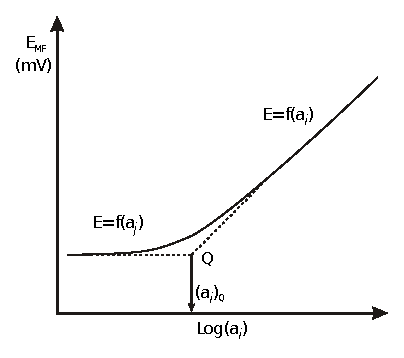
\includegraphics{ion1.eps}
\caption{Ionszelektív elektród szelektivitási együtthatójának meghatározása kevert oldatos módszerrel kapott adatokból.}
\label{fig:Q}
\end{figure}

A külön oldatos eljárás alkalmazásakor két görbe felvételére van szükség.
Zérus zavaró ion aktivitás mellett fel kell venni az elsődleges $i$ ionra vonatkozó kalibrációs görbét, majd egy másik mérés során zérus elsődleges ion aktivitás mellett meg kell határozni a $j$ zavaró ionra vonatkozó kalibrációs görbét.
Amint a 2. ábra mutatja, a két görbe segítségével a szelektivitási együttható értéke meghatározható az

\begin{enumerate}[(a)]
\item azonos poteniálokhoz tartozó aktivitások arányából

\begin{equation}
\label{eq:azonospot}
        k_{i,j}^{pot}
        =
        \frac{a_i}{a_j^{z_i/z_j}}
\end{equation}

\item az azonos aktivitásokhoz tartozó potenciálokból:

\begin{equation}
\label{eq:azonosakt}
        \lg k_{i,j}^{pot}
        =
        \frac{(E_2-E_1)zF}{2.303RT}
	=
	\frac{\Delta E}{S}
\end{equation}

\end{enumerate}

A szelektivitási együttható értékét számos tényező befolyásolja: a mintaoldat ionerőssége, a meghatározás módja, stb.
Látható az \ref{eq:azonospot}. és \ref{eq:azonosakt}. összefüggésekből a külön oldatos módszer hátránya: feltételezi, hogy az elsődleges és zavaró ionok töltése megegyezik, továbbá hogy az elektród meredeksége mindkét ionra azonos.
A külön oldatos módszernél a meghatározás körülményei a gyakorlatban felmerülő analízis körülményeitől eltérhetnek, ezért az így meghatározott szelektivitási együttható értékek közelítő értékeknek tekinthetők.

\begin{figure}
\centering
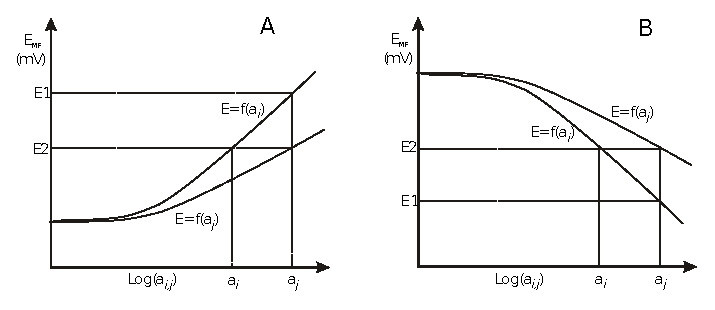
\includegraphics{ion2.eps}
\caption{A szelektivitási együtthatók meghatározása külön oldatos módszerrel. (A) Egyszeresen pozitív, és (B) egyszeresen negatív töltésű ionokra.}
\label{fig:ion2}
\end{figure}

\subsection{A gyakorlat leírása}
A gyakorlat célja a kálium-ion vagy fluorid-ion (kérdezze a gyakorlatvezetőtől) szelektív elektród funkcióinak vizsgálata.
Első feladatként meg kell határozni, hogy az elektród milyen aktivitástól képes – a Nernst egyenletnek megfelelően – az elsődleges ion aktivitásának mérésére.
Ehhez hígítási sort készítünk a megfelelő elsődleges ion sójából (KCl ill. NaF).
100 ml mérőlombikban készítsen 10$^{-2}$ mol$\cdot$dm$^{-3}$ koncentrációjú oldatot az elsődleges ion sójából.
10-szeres hígításhoz 10 ml-t pipettázzon át egy másik 100 ml mérőlombikba, és töltse jelre ioncserélt vízzel.
A hígítást addig ismételje új mérőlombikban mindig az előző oldatot felhasználva, míg el nem éri a 10$^{-6}$ mol$\cdot$dm$^{-3}$ koncentrációt.
Az oldatokat öntsük ki feliratozott főzőpoharakba.
Az elektródot a leghígabb oldatot tartalmazó edénybe merítjük a vonatkoztatási elektróddal együtt és csatlakoztatjuk a pH mérő megfelelő bemeneteihez.
Kb. 1 perc elteltével olvassuk le és jegyezzük fel az elektródpotenciál értékeket.
Leolvasás után merítsük az elektródokat a következő, tízszer töményebb oldatba és ismét 1 perc elteltével olvassuk le az elektródpotenciál értéket.
A mérést végezzük el mind az öt oldatban, a leghígabbtól a legtöményebb felé haladva háromszor egymás után.
A mérési sorozatok között és után alaposan öblítsük le az elektródot és a mérőedényt mossuk ki ioncserélt vízzel.

\subsubsection{A szelektivitási együttható meghatározása kevert oldatos eljárással}

A továbbiakban ismételjük meg a mérést, azonban a hígítási sor készítéséhez ioncserélt víz helyett 10$^{-2}$ mol$\cdot$dm$^{-3}$ koncentrációjú NaCl, oldatot használjunk (zavaró ion Na$^+$, illetve Cl$^-$ a K$^+$, illetve F$^-$ ion-szelektív elektród esetére).
Mivel a mérésekkor termosztálást nem alkalmaztunk, jegyezzük fel a laboratórium hőmérsékletét.
Fontos, hogy az oldatok készítéséhez kálium, nátrium, klorid és fluorid ionoktól mentes vizet használjunk.

\subsubsection{A szelektivitási együttható különoldatos eljárással}

Az elektródok leöblítése után határozzuk meg az elektród szelektivitási együtthatóját külön oldatos módszerrel.
Ehhez a zavaró ion sójából készítünk hígítási sort, a 2. pont bevezetésében leírt módszerrel.
Mivel a zavaró ionra az ion-szelektív elektród (ideálisan) sokkal kevésbé érzékeny, ezért nagyobb koncentrációt kell alkalmaznunk, hogy vizsgálhassuk a zavaró hatást.
A mérés befejeztével öblítsük le az elektródot és a mérőedényt mossuk ki ioncserélt vízzel.

\subsection{A gyakorlat kiértékelése}

A koncentrációk, aktivitási koefficiensek és a térfogat értékek ismeretében számítsa ki az oldatok elsődleges ion aktivitását.
Ábrázolja a mért potenciálértékeket az elsődleges ion aktivitás logaritmusának függvényében.

A kevert oldatos mérések során felvett, a különböző oldatokban nyert görbéket ábrázolja egy diagramban.
Határozza meg minden mérési sorozatból az elektród meredekségét.
A csak elsődleges ionok jelenlétében felvett görbéből határozza meg a grafikusan az elektród kimutatási határát is.

A kevert oldatos mérésekből az 1. ábrán bemutatott módon határozza meg a (4) egyenlet alkalmazásával a szelektivitási együttható értékeit a különböző klorid ion aktivitások mellett.
Ábrázolja a szelektivitási együttható értékét a kloridion aktivitás függvényében.

A különoldatos módszerrel történő kiértékeléshez egy diagramban ábrázolja az elektród potenciált az illető ion aktivitásának függvényében (egyszer az elsődleges, egyszer a zavaró ion esetén).
Figyelembe kell vennie, hogy a közepes aktivitási koefficiensek eltérőek lehetnek.
A két görbéből a 2. ábrának megfelelően két, azonos aktivitáshoz tartozó potenciálnál, valamint azonos potenciálhoz tartozó két aktivitásból is számítsa ki a szelektivitási együttható értékét.

\subsection{Beadandó eredmények}
Az elektród kimutatási határa, 3 szelektivitási együttható kevert, és 2 szelektivitási együttható külön oldatos módszerrel meghatározva.
Az elektród meredeksége azelsődleges ill. a zavaró ionokat tartalmazó oldatban. 5 kalibrációs görbe.

